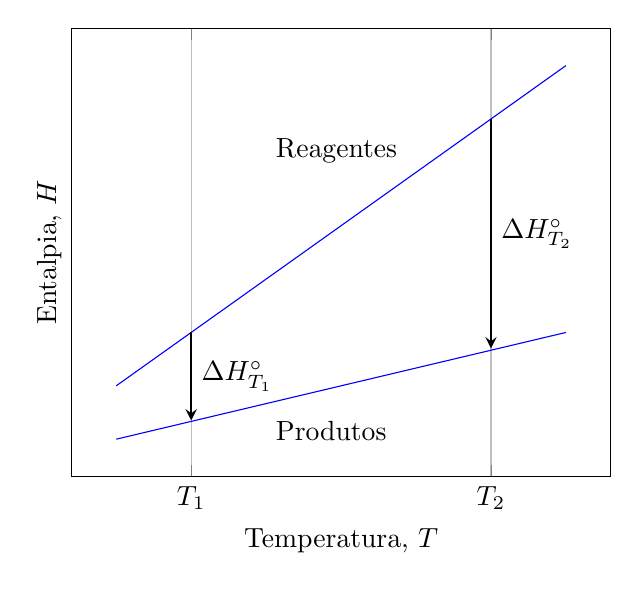
\begin{tikzpicture}
    \begin{axis}
        [
            grid = major,
            xlabel = {Temperatura, $T$},
            ylabel = {Entalpia, $H$},
            ytick=\empty,  
            xtick={1.5,3.5},
            xticklabels={$T_1$,$T_2$},
        ]
    \addplot [blue] coordinates
        {
            (1,2)
            (4,8)
        };
    \addplot [blue] coordinates
        {
            (1,1)
            (4,3)
        };
    \draw [ draw=black, thick, -stealth ]
        (axis cs: 1.5, 3) -- node [right] {$\Delta H_{T_1}^\circ$}
        (axis cs: 1.5, 1.35);
    \draw [ draw=black, thick, -stealth ]
        (axis cs: 3.5, 7) -- node [right] {$\Delta H_{T_2}^\circ$}
        (axis cs: 3.5, 2.7);
    \node [anchor = south west] at (axis cs:2,6) 
        {Reagentes};
    \node [anchor = south west] at (axis cs:2,0.8) 
        {Produtos};
    \end{axis}
\end{tikzpicture}